
\documentclass{article}
%\usepackage[utf8]{inputeatbibc}
\usepackage{amsmath}
\usepackage{graphicx}
\usepackage{comment}
\usepackage[colorinlistoftodos]{todonotes}
\usepackage[colorlinks=true, allcolors=blue]{hyperref}
\usepackage[english]{babel}
\usepackage[T1]{fontenc}
\usepackage[a4paper,top=3cm,bottom=2cm,left=3cm,right=3cm,marginparwidth=1.75cm]{geometry}
\usepackage{listings}
\usepackage{biblatex}
\usepackage{url}
\usepackage{hyperref}
\addbibresource{proposal.bib}
% Fundamental packages
\usepackage[utf8]{inputenc}
\usepackage{lmodern}
\usepackage[T1]{fontenc}
%\usepackage{soul}
%\usepackage{natbib}




\begin{document}

\begin{titlepage}
\begin{center}
\vspace{1cm}

\includegraphics[scale=0.5]{Logo_EPFL.png}\par
\vspace{4cm}

{\Huge \bf Research Proposal \par}




\vspace{3cm}

{\large Aurélien Morel, Lucas Waelti \& Luca Kiener}\par
\vspace{2cm}

\today


\vfill
\end{center}
\end{titlepage}

\section{Scientific Question}
The model of the salamander that we used in our previous experiments gave really good results for a stable swimming gait in still water. This led us to ask ourselves another question: how does the animal deal with current? More precisely, how does it keep a stable straight trajectory when it is subject to sideways current? We would like both to understand how the real animal behaves and how we could create a model that mimics the animal's behavior. 

\section{Hypothesis}
We know that the real salamander has pressure sensitive cells on its skin to provide some sensory feedback to the spinal cord. It is also known that the animal uses the feedback to sense the current. Our hypothesis is that this information has direct influence on the spinal cord patterns. Furthermore, we think that the salamander's brain does not have any influence: the animal keeps the same drive (trying to go straight) but the sensory inputs and the spinal cord's neuron network are sufficient to provide the adaptation to the current. 

\section{Experiments}
In order to test our hypothesis, we would like to propose two experiments to be run sequentially: first one on a real salamander and one on our simulation model. 
\begin{figure}[!ht]
    \centering
    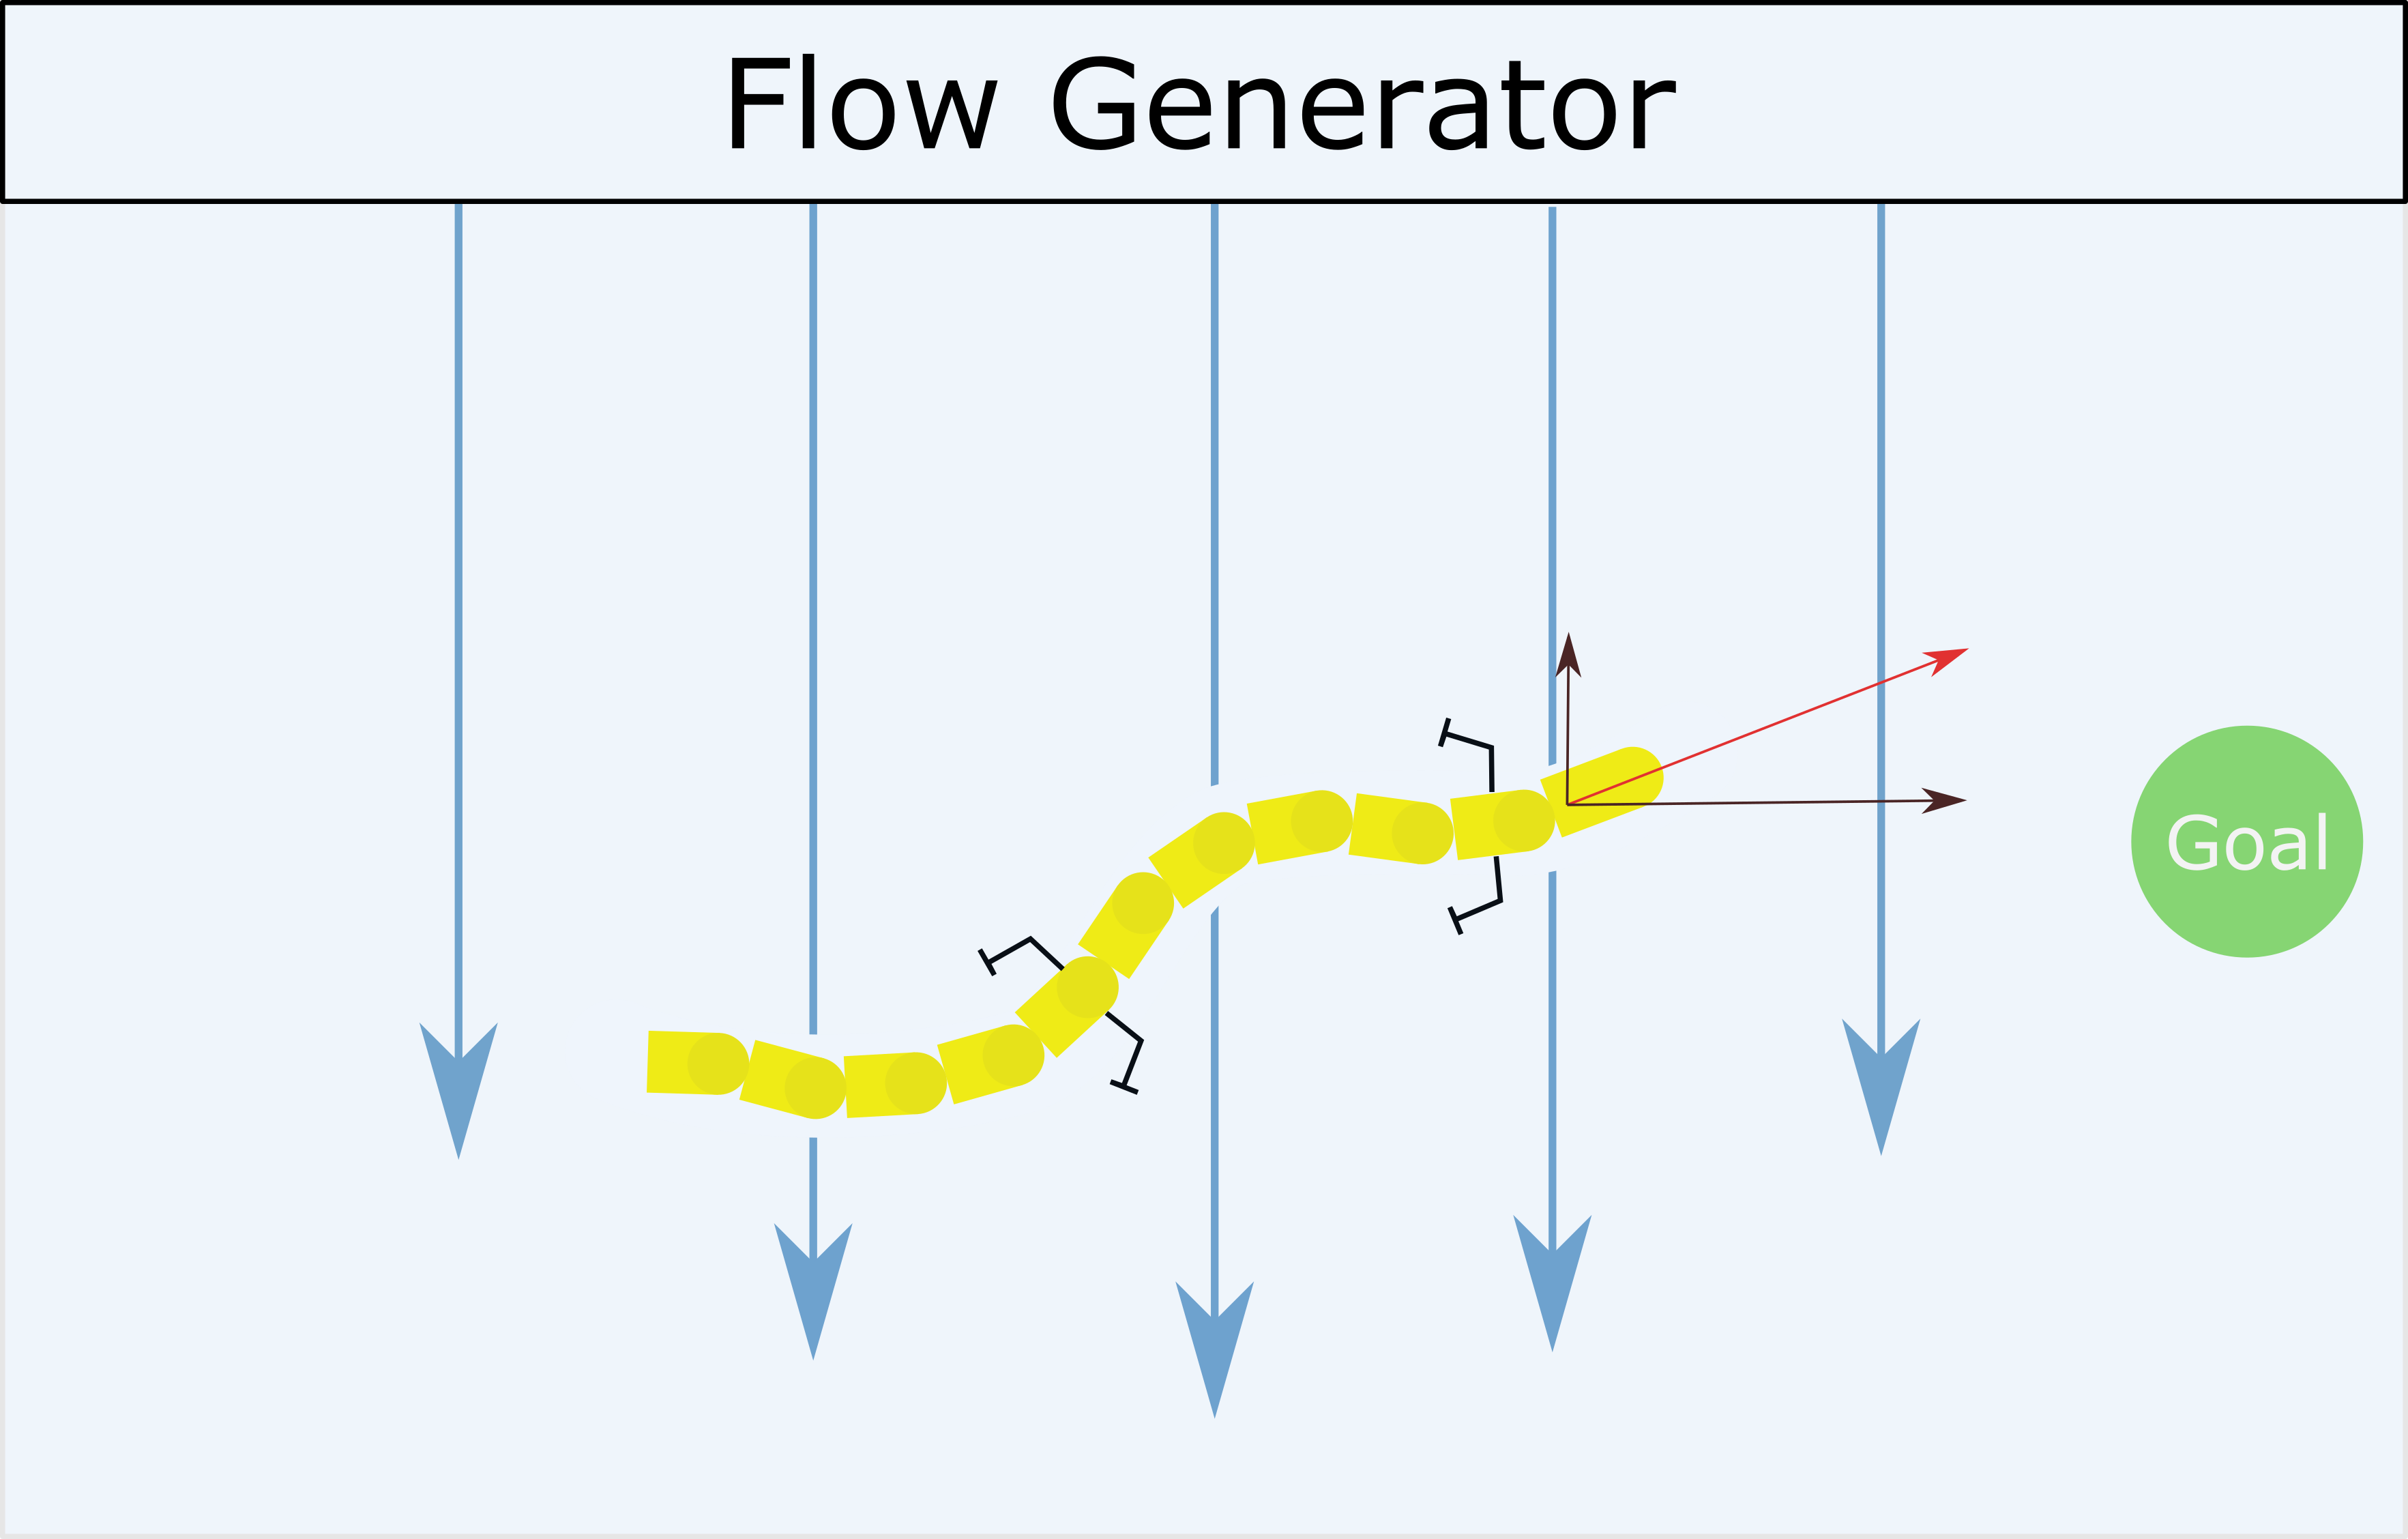
\includegraphics[width=0.6\textwidth]{flow.png}
    \caption{Experimental Setup}
    \label{setup}
\end{figure}

\subsection{Real Salamander Experiment}
Our experiment on a the real animal would be really simple. We just need a pool that can produce a constant current and a camera. The goal would be to install the camera on the top of the pool facing downwards and lure the salamander to go through the pool, with current on its side. When the data is collected, we would use computer vision techniques to track the animal and study its trajectory. This would provide us ground truth on how the salamander deals with sideways current. 


\subsection{Simulation Model Experiment}
Having the results from the real world experiment, the goal of the simulation would be to try to \textbf{reproduce the behavior} on the salamander on our model by using coupling of the sensory feedback to the spinal cord network. The simulation would use our previous model that combines neural modelling and biomechanical modelling (neuromechanical model). In order to do this, we would first need to implement the pressure sensors on the sides of the robot. More precisely, there would be a pressure sensor on both sides of each link and directly coupled to both oscillators (Figure \ref{Network}) similar to the segmental neuronal network in a lamprey \cite{GRILLNER1995270} or the cutaneous feedback in a cat limb \cite{frigon06}. Then, we would implement the coupling (i.e. ipsilateral excitatory and contralateral inhibitatory coupling \cite{GRILLNER1995270}). Also, we would need to model the environment by adding a constant velocity to the liquid. The final step would be to vary the coupling parameters and simulate the model in our environment \textbf{without changing the drive} until we find values that lead to a behavior that is close to the natural one. 

\begin{figure}[h]
    \centering
    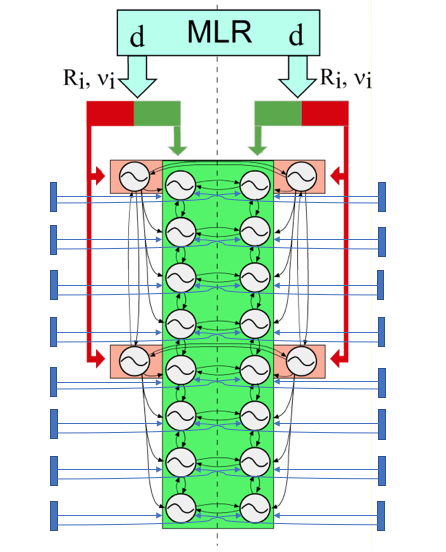
\includegraphics[scale=0.5]{New_Network.png}
    \caption{CPG model with additional pressure sensor couplings (blue). Mesencephalic Locomotor Region (MLR) setting the drive (d), which sets the nominal amplitude ($R_i$) and frequency ($v_i$) of the network.}
    \label{Network}
\end{figure}

\subsection{Expected Results and Interpretation}

If we find such parameters value, it would prove that it is indeed possible to deal with sideways current without having any influence of the brain. 

However, this would not prove that it is how the salamander does it in real life. In order to tackle this question, we would need to plan another experiment on a real salamander. Indeed, we would use the same real world setup but we would need to find a way to cut out the influence of the brain and manually apply electrical stimulation to the spine, either using medical or surgical techniques. 



%\section{Links}
%Link to the papers on moodle: %\url{https://moodle.epfl.ch/mod/folder/view.php?id=1020123}

%\url{https://moodle.epfl.ch/pluginfile.php/2646188/mod_folder/content/0/frigon06.pdf?forcedownload=1}

%\url{https://moodle.epfl.ch/pluginfile.php/2646188/mod_folder/content/0/Pearson_et_al_2006_sensory_fct_neuromech_sim.pdf?forcedownload=1}

%\url{https://moodle.epfl.ch/pluginfile.php/2646188/mod_folder/content/0/Markin_et_al_2016_Neuromechanical_model_of_cat_Rybak.pdf?forcedownload=1}




%\newpage

%\bibliographystyle{ieeetr}
%\bibliography{proposal}
%\label{sec:references}

\printbibliography




\end{document}

